% Options for packages loaded elsewhere
% Options for packages loaded elsewhere
\PassOptionsToPackage{unicode}{hyperref}
\PassOptionsToPackage{hyphens}{url}
%
\documentclass[
  ignorenonframetext,
]{beamer}
\newif\ifbibliography
\usepackage{pgfpages}
\setbeamertemplate{caption}[numbered]
\setbeamertemplate{caption label separator}{: }
\setbeamercolor{caption name}{fg=normal text.fg}
\beamertemplatenavigationsymbolsempty
% remove section numbering
\setbeamertemplate{part page}{
  \centering
  \begin{beamercolorbox}[sep=16pt,center]{part title}
    \usebeamerfont{part title}\insertpart\par
  \end{beamercolorbox}
}
\setbeamertemplate{section page}{
  \centering
  \begin{beamercolorbox}[sep=12pt,center]{section title}
    \usebeamerfont{section title}\insertsection\par
  \end{beamercolorbox}
}
\setbeamertemplate{subsection page}{
  \centering
  \begin{beamercolorbox}[sep=8pt,center]{subsection title}
    \usebeamerfont{subsection title}\insertsubsection\par
  \end{beamercolorbox}
}
% Prevent slide breaks in the middle of a paragraph
\widowpenalties 1 10000
\raggedbottom
\AtBeginPart{
  \frame{\partpage}
}
\AtBeginSection{
  \ifbibliography
  \else
    \frame{\sectionpage}
  \fi
}
\AtBeginSubsection{
  \frame{\subsectionpage}
}
\usepackage{iftex}
\ifPDFTeX
  \usepackage[T1]{fontenc}
  \usepackage[utf8]{inputenc}
  \usepackage{textcomp} % provide euro and other symbols
\else % if luatex or xetex
  \usepackage{unicode-math} % this also loads fontspec
  \defaultfontfeatures{Scale=MatchLowercase}
  \defaultfontfeatures[\rmfamily]{Ligatures=TeX,Scale=1}
\fi
\usepackage{lmodern}

\ifPDFTeX\else
  % xetex/luatex font selection
\fi
% Use upquote if available, for straight quotes in verbatim environments
\IfFileExists{upquote.sty}{\usepackage{upquote}}{}
\IfFileExists{microtype.sty}{% use microtype if available
  \usepackage[]{microtype}
  \UseMicrotypeSet[protrusion]{basicmath} % disable protrusion for tt fonts
}{}
\makeatletter
\@ifundefined{KOMAClassName}{% if non-KOMA class
  \IfFileExists{parskip.sty}{%
    \usepackage{parskip}
  }{% else
    \setlength{\parindent}{0pt}
    \setlength{\parskip}{6pt plus 2pt minus 1pt}}
}{% if KOMA class
  \KOMAoptions{parskip=half}}
\makeatother

\usepackage{color}
\usepackage{fancyvrb}
\newcommand{\VerbBar}{|}
\newcommand{\VERB}{\Verb[commandchars=\\\{\}]}
\DefineVerbatimEnvironment{Highlighting}{Verbatim}{commandchars=\\\{\}}
% Add ',fontsize=\small' for more characters per line
\usepackage{framed}
\definecolor{shadecolor}{RGB}{241,243,245}
\newenvironment{Shaded}{\begin{snugshade}}{\end{snugshade}}
\newcommand{\AlertTok}[1]{\textcolor[rgb]{0.68,0.00,0.00}{#1}}
\newcommand{\AnnotationTok}[1]{\textcolor[rgb]{0.37,0.37,0.37}{#1}}
\newcommand{\AttributeTok}[1]{\textcolor[rgb]{0.40,0.45,0.13}{#1}}
\newcommand{\BaseNTok}[1]{\textcolor[rgb]{0.68,0.00,0.00}{#1}}
\newcommand{\BuiltInTok}[1]{\textcolor[rgb]{0.00,0.23,0.31}{#1}}
\newcommand{\CharTok}[1]{\textcolor[rgb]{0.13,0.47,0.30}{#1}}
\newcommand{\CommentTok}[1]{\textcolor[rgb]{0.37,0.37,0.37}{#1}}
\newcommand{\CommentVarTok}[1]{\textcolor[rgb]{0.37,0.37,0.37}{\textit{#1}}}
\newcommand{\ConstantTok}[1]{\textcolor[rgb]{0.56,0.35,0.01}{#1}}
\newcommand{\ControlFlowTok}[1]{\textcolor[rgb]{0.00,0.23,0.31}{\textbf{#1}}}
\newcommand{\DataTypeTok}[1]{\textcolor[rgb]{0.68,0.00,0.00}{#1}}
\newcommand{\DecValTok}[1]{\textcolor[rgb]{0.68,0.00,0.00}{#1}}
\newcommand{\DocumentationTok}[1]{\textcolor[rgb]{0.37,0.37,0.37}{\textit{#1}}}
\newcommand{\ErrorTok}[1]{\textcolor[rgb]{0.68,0.00,0.00}{#1}}
\newcommand{\ExtensionTok}[1]{\textcolor[rgb]{0.00,0.23,0.31}{#1}}
\newcommand{\FloatTok}[1]{\textcolor[rgb]{0.68,0.00,0.00}{#1}}
\newcommand{\FunctionTok}[1]{\textcolor[rgb]{0.28,0.35,0.67}{#1}}
\newcommand{\ImportTok}[1]{\textcolor[rgb]{0.00,0.46,0.62}{#1}}
\newcommand{\InformationTok}[1]{\textcolor[rgb]{0.37,0.37,0.37}{#1}}
\newcommand{\KeywordTok}[1]{\textcolor[rgb]{0.00,0.23,0.31}{\textbf{#1}}}
\newcommand{\NormalTok}[1]{\textcolor[rgb]{0.00,0.23,0.31}{#1}}
\newcommand{\OperatorTok}[1]{\textcolor[rgb]{0.37,0.37,0.37}{#1}}
\newcommand{\OtherTok}[1]{\textcolor[rgb]{0.00,0.23,0.31}{#1}}
\newcommand{\PreprocessorTok}[1]{\textcolor[rgb]{0.68,0.00,0.00}{#1}}
\newcommand{\RegionMarkerTok}[1]{\textcolor[rgb]{0.00,0.23,0.31}{#1}}
\newcommand{\SpecialCharTok}[1]{\textcolor[rgb]{0.37,0.37,0.37}{#1}}
\newcommand{\SpecialStringTok}[1]{\textcolor[rgb]{0.13,0.47,0.30}{#1}}
\newcommand{\StringTok}[1]{\textcolor[rgb]{0.13,0.47,0.30}{#1}}
\newcommand{\VariableTok}[1]{\textcolor[rgb]{0.07,0.07,0.07}{#1}}
\newcommand{\VerbatimStringTok}[1]{\textcolor[rgb]{0.13,0.47,0.30}{#1}}
\newcommand{\WarningTok}[1]{\textcolor[rgb]{0.37,0.37,0.37}{\textit{#1}}}

\usepackage{longtable,booktabs,array}
\newcounter{none} % for unnumbered tables
\usepackage{calc} % for calculating minipage widths
\usepackage{caption}
% Make caption package work with longtable
\makeatletter
\def\fnum@table{\tablename~\thetable}
\makeatother
\usepackage{graphicx}
\makeatletter
\newsavebox\pandoc@box
\newcommand*\pandocbounded[1]{% scales image to fit in text height/width
  \sbox\pandoc@box{#1}%
  \Gscale@div\@tempa{\textheight}{\dimexpr\ht\pandoc@box+\dp\pandoc@box\relax}%
  \Gscale@div\@tempb{\linewidth}{\wd\pandoc@box}%
  \ifdim\@tempb\p@<\@tempa\p@\let\@tempa\@tempb\fi% select the smaller of both
  \ifdim\@tempa\p@<\p@\scalebox{\@tempa}{\usebox\pandoc@box}%
  \else\usebox{\pandoc@box}%
  \fi%
}
% Set default figure placement to htbp
\def\fps@figure{htbp}
\makeatother





\setlength{\emergencystretch}{3em} % prevent overfull lines

\providecommand{\tightlist}{%
  \setlength{\itemsep}{0pt}\setlength{\parskip}{0pt}}



 


\makeatletter
\@ifpackageloaded{caption}{}{\usepackage{caption}}
\AtBeginDocument{%
\ifdefined\contentsname
  \renewcommand*\contentsname{Table of contents}
\else
  \newcommand\contentsname{Table of contents}
\fi
\ifdefined\listfigurename
  \renewcommand*\listfigurename{List of Figures}
\else
  \newcommand\listfigurename{List of Figures}
\fi
\ifdefined\listtablename
  \renewcommand*\listtablename{List of Tables}
\else
  \newcommand\listtablename{List of Tables}
\fi
\ifdefined\figurename
  \renewcommand*\figurename{Figure}
\else
  \newcommand\figurename{Figure}
\fi
\ifdefined\tablename
  \renewcommand*\tablename{Table}
\else
  \newcommand\tablename{Table}
\fi
}
\@ifpackageloaded{float}{}{\usepackage{float}}
\floatstyle{ruled}
\@ifundefined{c@chapter}{\newfloat{codelisting}{h}{lop}}{\newfloat{codelisting}{h}{lop}[chapter]}
\floatname{codelisting}{Listing}
\newcommand*\listoflistings{\listof{codelisting}{List of Listings}}
\makeatother
\makeatletter
\makeatother
\makeatletter
\@ifpackageloaded{caption}{}{\usepackage{caption}}
\@ifpackageloaded{subcaption}{}{\usepackage{subcaption}}
\makeatother

\usepackage{bookmark}
\IfFileExists{xurl.sty}{\usepackage{xurl}}{} % add URL line breaks if available
\urlstyle{same}
% fallback for those not using the hyperref driver hyperxmp:
\makeatletter
\@ifundefined{xmpquote}{\newcommand{\xmpquote}[1]{#1}}{}
\makeatother
\hypersetup{
  pdftitle={Probability},
  hidelinks,
  pdfcreator={LaTeX via pandoc}}


\title{\texorpdfstring{Probability}{Probability}}
\subtitle{\texorpdfstring{Random Variables, Probability
Distributions}{Random Variables, Probability Distributions}}
\author{}
\date{}

\begin{document}
\frame{\titlepage}


\begin{frame}{Sampling}
\protect\phantomsection\label{sampling}
A {Simple Random Sample} (SRS) of size \(n\) from a finite population is
a subset selected in such a way that every subset of n elements is
equally likely to be the one selected.
\end{frame}

\begin{frame}{Random Variables}
\protect\phantomsection\label{random-variables}
A {random variable} is a function defined on a numeric population. We
often say that this function value is the value assumed by the random
variable. A probability distribution specifies the probabilities
associated with all possible values the random variable can assume.
\end{frame}

\begin{frame}{Example}
\protect\phantomsection\label{example}
If \(X\) represents the number of RED \(M\&Ms\) in a vending machine
size package, then perhaps {the probability distribution of \(X\)} is
something like the following:\\

{\def\LTcaptype{none} % do not increment counter
\begin{longtable}[]{@{}cccccccc@{}}
\toprule\noalign{}
\(x\) & 5 & 6 & 7 & 8 & 9 & 10 & 11 \\
\midrule\noalign{}
\endhead
\(P(X=x)\) & \(\frac{2}{28}\) & \(\frac{2}{28}\) & \(\frac{5}{28}\) &
\(\frac{7}{28}\) & \(\frac{5}{28}\) & \(\frac{4}{28}\) &
\(\frac{3}{28}\) \\
\bottomrule\noalign{}
\end{longtable}
}
\end{frame}

\begin{frame}
\pandocbounded{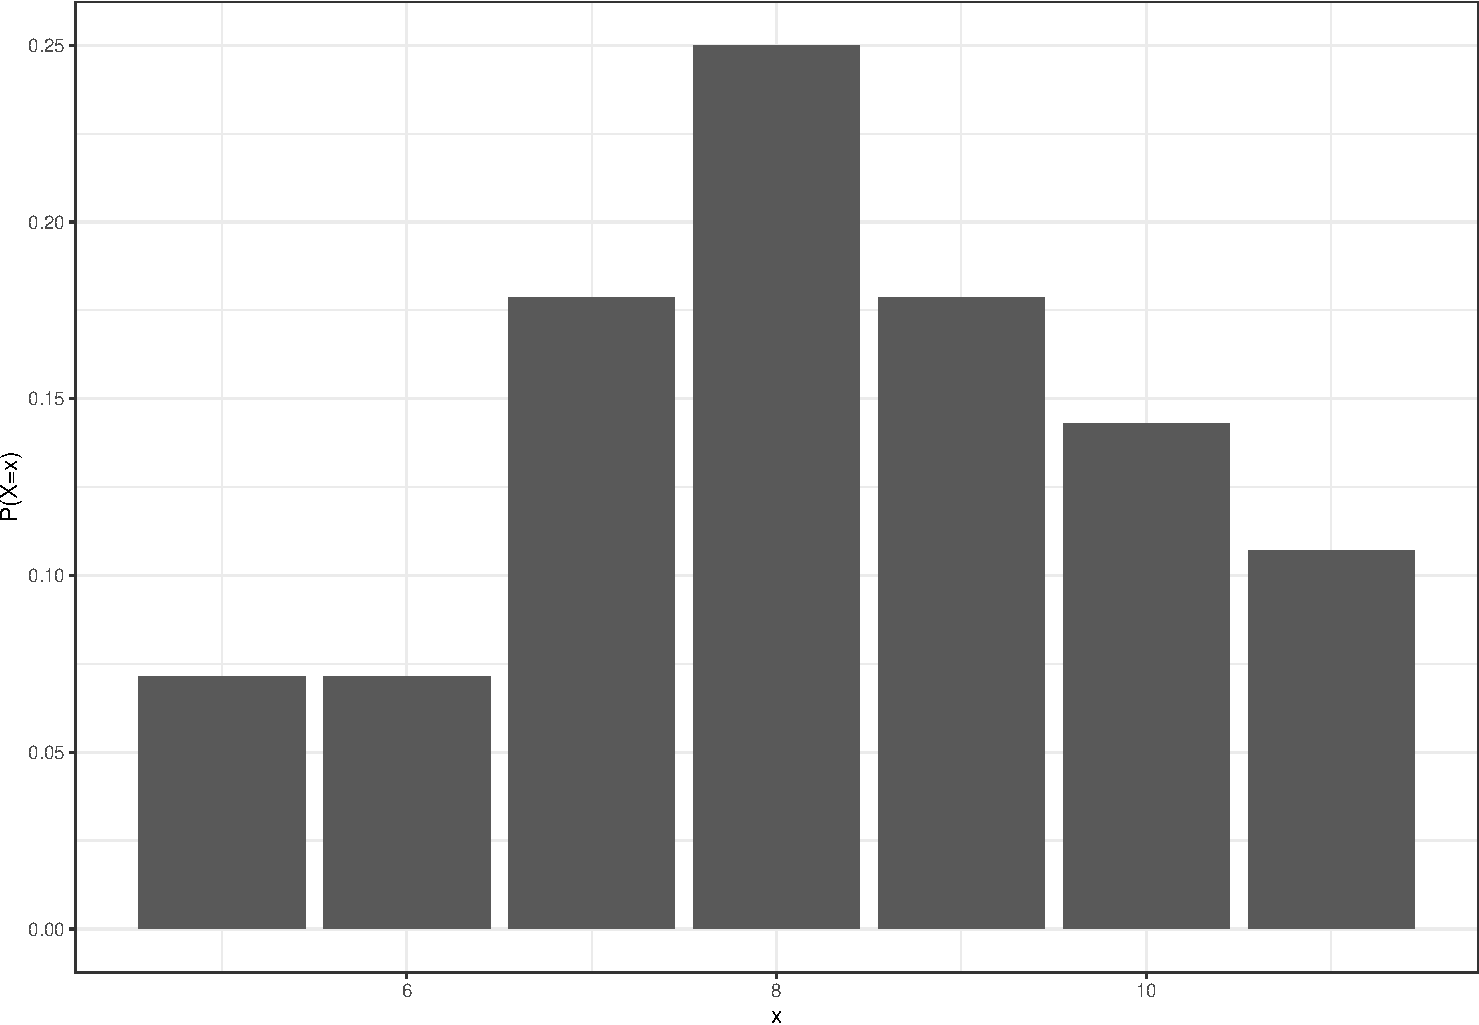
\includegraphics[keepaspectratio]{part2_inclass_files/figure-beamer/unnamed-chunk-1-1.pdf}}
\end{frame}

\begin{frame}{Discrete Random Variables}
\protect\phantomsection\label{discrete-random-variables}
When the elements of a population consists of a countable discrete set
of values the random variable defined on that population is called
discrete random variable.

Properties:

\begin{itemize}
\tightlist
\item
  \(0\leq P(X=x)\) for all x
\item
  \(\sum_x P(X=x)=1\)
\end{itemize}
\end{frame}

\begin{frame}[fragile]{Continuous Random Variables}
\protect\phantomsection\label{continuous-random-variables}
When the population consists of a set of values in a continuous range
the random variable defined on that population is called continuous
random variable. The probability distribution of a continuous random
variable is a smooth curve, and the area under the curve between
specified values of the random value correspond to a probability.

\begin{Shaded}
\begin{Highlighting}[]
\NormalTok{x }\OtherTok{\textless{}{-}} \FunctionTok{seq}\NormalTok{(}\SpecialCharTok{{-}}\DecValTok{4}\NormalTok{,}\DecValTok{4}\NormalTok{, }\AttributeTok{l =} \DecValTok{1000}\NormalTok{)}
\FunctionTok{ggplot}\NormalTok{(}\AttributeTok{mapping =} \FunctionTok{aes}\NormalTok{(}\AttributeTok{x =}\NormalTok{ x,}
                     \AttributeTok{y =} \FunctionTok{dnorm}\NormalTok{(x))) }\SpecialCharTok{+} 
  \FunctionTok{geom\_path}\NormalTok{() }\SpecialCharTok{+} 
  \FunctionTok{theme\_void}\NormalTok{()}
\end{Highlighting}
\end{Shaded}

\begin{center}
\pandocbounded{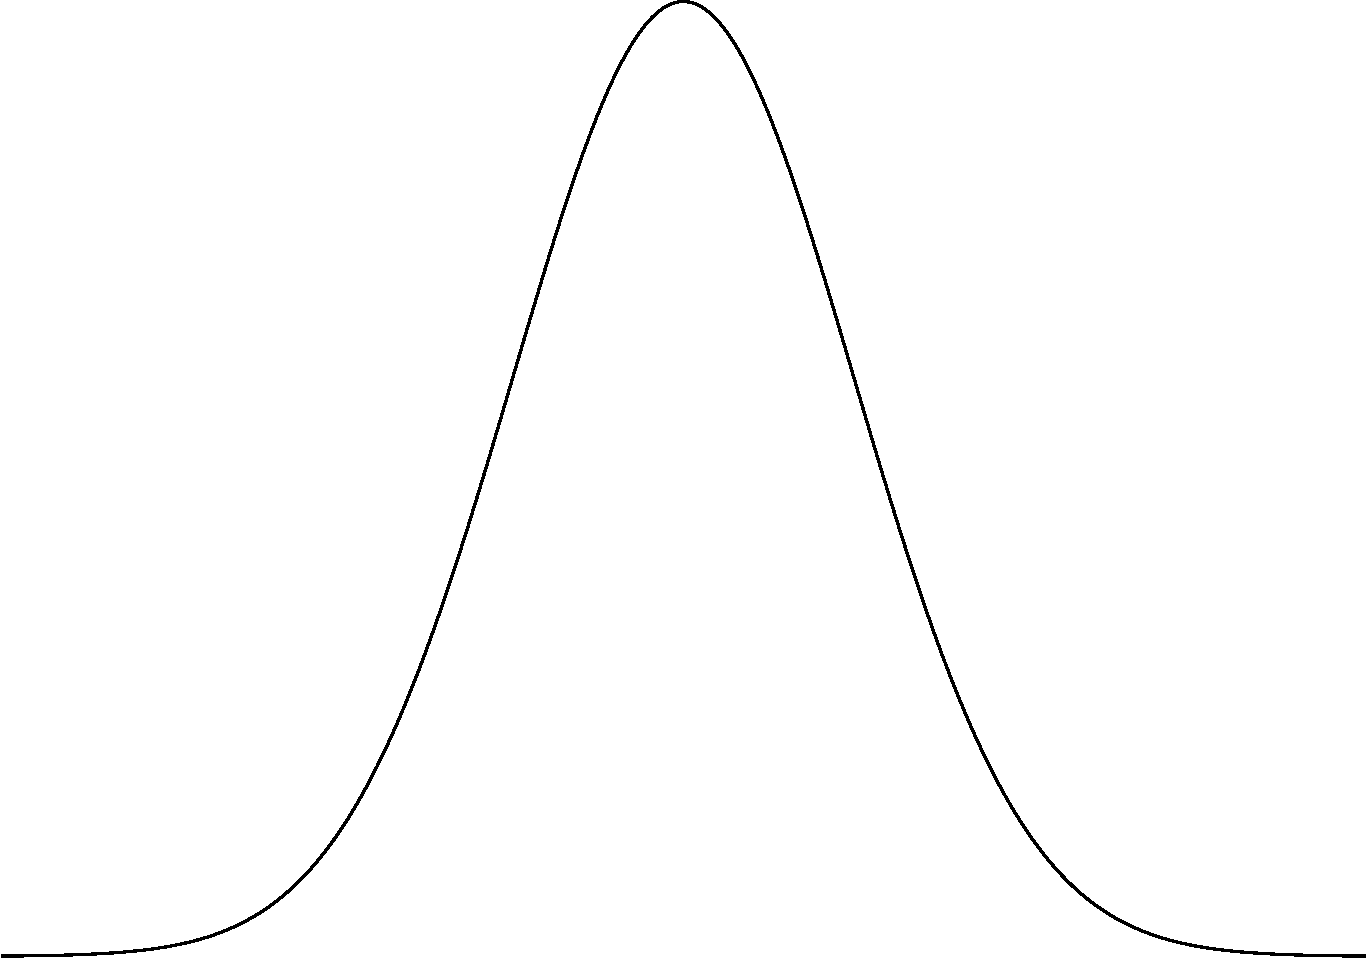
\includegraphics[keepaspectratio]{part2_inclass_files/figure-beamer/unnamed-chunk-2-1.pdf}}
\end{center}
\end{frame}

\begin{frame}{Continuous RV (example)}
\protect\phantomsection\label{continuous-rv-example}
Suppose that our population consists of all numbers in the interval
(0,2) occurring with various frequencies as specified by \(f(x)\).

\hfill\break
\hfill\break
\hfill\break
\hfill\break
\hfill\break

\begin{itemize}
\tightlist
\item
  \(P(1/2\leq X\leq 1/2)=\)
\end{itemize}

\hfill\break
\hfill\break
\hfill\break

\begin{itemize}
\tightlist
\item
  \(P(0\leq X\leq 2)=\)
\end{itemize}

\hfill\break
\hfill\break
\hfill\break

\begin{itemize}
\tightlist
\item
  \(P(1\leq X\leq 2)=\)
\end{itemize}
\end{frame}

\begin{frame}{Common Distributions}
\protect\phantomsection\label{common-distributions}
For some interesting populations that occur naturally, theoretical
probability distributions and associated random variables, have been
defined.

Discrete

\begin{itemize}
\tightlist
\item
  Binomial
\item
  Poisson
\item
  Negative Binomial
\end{itemize}

Continuous

\begin{itemize}
\tightlist
\item
  Normal
\item
  Gamma
\item
  Chi squared
\item
  F
\item
  t
\end{itemize}
\end{frame}

\begin{frame}{Binomial Experiment}
\protect\phantomsection\label{binomial-experiment}
A binomial experiment consists of taking \(n\) successive SRS, each of
size 1, replacing elements between draws, and counting the number of
``successes'' (S) obtained, \(m\). The alternative is ``failures'' (F).

\begin{itemize}
\tightlist
\item
  \(\pi=m/n\)
\item
  \(1-\pi=(N-m)/N\)
\end{itemize}

Let \(X_i\) be the random variable that assumes the value of the outcome
of the \(i\)-th draw for each \(i=1,2,\dots,n\).
\end{frame}

\begin{frame}{Binomial Distribution}
\protect\phantomsection\label{binomial-distribution}
Let \(X_i\) assume the value 1 if the outcome of the \(i\)-th draw is S
or the value of 0 if the outcome is F. For a repeated process, \(n\)
random variables, \(X_1,X_2,\dots,X_n\), are distributed as follows:

{\def\LTcaptype{none} % do not increment counter
\begin{longtable}[]{@{}ccc@{}}
\toprule\noalign{}
\(x\) & 0 & 1 \\
\midrule\noalign{}
\endhead
\(P(X=x)\) & \(1-\pi\) & \(\pi\) \\
\bottomrule\noalign{}
\end{longtable}
}
\end{frame}

\begin{frame}{Binomial Distribution (contd.)}
\protect\phantomsection\label{binomial-distribution-contd.}
Now define a new random variable \(Y\) so that

\[Y = X_1 + X_2 + X_3 + \cdots + X_n\]

\begin{itemize}
\tightlist
\item
  \(Y\) represents the number of ``successes'' for the \(n\) random
  variables
\item
  \(Y\) is said to be a binomial random variable.
\end{itemize}
\end{frame}

\begin{frame}{Binomial Distribution (contd.)}
\protect\phantomsection\label{binomial-distribution-contd.-1}
\[
Y\sim \text{Binomial}(n,\pi);\quad y=1,2,\dots,n; \quad 0\lt \pi\lt 1
\]

\hfill\break
\hfill\break
\hfill\break

\(P(Y=y)=\)
\end{frame}

\begin{frame}{Mean and Variance of a Discrete Random Variable}
\protect\phantomsection\label{mean-and-variance-of-a-discrete-random-variable}
\begin{itemize}
\item
  The {mean} of a discrete random variable \(X\) is:
  \[E(X) = \mu = \sum_x\,x \cdot P(X=x)\]
\item
  The {variance} of a discrete random variable \(X\) is:
  \[V(X) = \sigma^2= \sum_x\,(x - E(X))^2\cdot \ P(X=x)\]
\item
  The {standard deviation} of a random variable \(X\) is
  \[\sqrt{V(X)}=\sigma\]
\end{itemize}
\end{frame}

\begin{frame}{Mean and Variance of a Discrete Random Variable (contd.)}
\protect\phantomsection\label{mean-and-variance-of-a-discrete-random-variable-contd.}
\begin{itemize}
\item
  Using the previous formula, the {mean} of a Binomial random variable
  \(Y\), is shown to be \(E(Y)=\mu = n \pi\)
\item
  The {variance} is shown to be \(V(Y) =\sigma^2= n\pi(1 - \pi)\).
\item
  Thus the {standard deviation} of a Binomial random variable is
  \(\sigma= \sqrt{n\,\pi(1 - \pi)}\)
\end{itemize}
\end{frame}

\begin{frame}{Binomial Distribution: Example}
\protect\phantomsection\label{binomial-distribution-example}
Consider a Binomial population where \(Y\sim Bin(3,1/3)\).

\begin{itemize}
\tightlist
\item
  Mean:
\end{itemize}

\hfill\break
\hfill\break
\hfill\break

\begin{itemize}
\tightlist
\item
  Variance:
\end{itemize}

\hfill\break
\hfill\break
\hfill\break

\begin{itemize}
\tightlist
\item
  Standard Deviation:
\end{itemize}
\end{frame}

\begin{frame}{Assumptions of the Binomial Model}
\protect\phantomsection\label{assumptions-of-the-binomial-model}
\begin{enumerate}
\item
  \(n\) identical trials are made.
\item
  Each trial results in either {Success(\(S\))} or {Failure(\(F\))}.
  (only two possible outcomes).
\item
  The probability of success (\(\pi\)) remains the same from trial to
  trial.
\item
  The trials are independent.
\item
  Interest is in the number of successes obtained in the \(n\) trials.
  The number is viewed as being the value assumed by a Binomial
  (\(n,\ \pi\)) random variable \(Y\).
\end{enumerate}
\end{frame}

\begin{frame}[fragile]{Binomial Distribution: R}
\protect\phantomsection\label{binomial-distribution-r}
Let \(Y\sim Bin(n,\pi)\)

\begin{itemize}
\tightlist
\item
  \(P(Y=y)\) is given by \texttt{dbinom(x=y,\ size=n,\ prob=pi)}
\item
  \(P(Y\leq y)\) is given by \texttt{pbinom(x=y,\ size=n,\ prob=pi)}
\end{itemize}
\end{frame}

\begin{frame}{Normal Random Variable}
\protect\phantomsection\label{normal-random-variable}
The Normal probability distribution is an example of a continuous
distribution, and is defined in the interval \(-\infty,\infty\). This is
a bell-shaped distribution and is commonly used to model continuous
data.

\(f(x)=\)

where

\begin{itemize}
\tightlist
\item
  \(E(X)=\)
\end{itemize}

\hfill\break

\begin{itemize}
\tightlist
\item
  \(V(X)=\)
\end{itemize}

\hfill\break

\begin{itemize}
\tightlist
\item
  \(\sqrt{V(X)}\)=
\end{itemize}
\end{frame}

\begin{frame}{Properties of the Normal Distribution}
\protect\phantomsection\label{properties-of-the-normal-distribution}
\begin{itemize}
\tightlist
\item
  Symmetric about the mean \(\mu\)
\item
  Probabilities calculated as
\end{itemize}

\[
P(a \leq X \leq b) = \frac{1}{\sqrt{2\pi}\sigma}\int_a^b e^{-\frac{1}{2}(\frac{x-\mu}{\sigma})^2} dx
\]
\end{frame}

\begin{frame}{Standard Normal Distribution}
\protect\phantomsection\label{standard-normal-distribution}
The standard normal distribution is a normal distribution with \(\mu=0\)
and \(\sigma^2=1\), and is represented by the random variable \(Z\). If
\(X\sim N(\mu,\sigma^2)\), then the following transformation converts
\(X\) into a standard normal random variable.

\[
Z=\frac{X-\mu}{\sigma}
\]
\end{frame}

\begin{frame}{Standard Normal Distribution}
\protect\phantomsection\label{standard-normal-distribution-1}
If \(X\sim N(0,\sigma^2)\), then we can use a Z-table to compute areas
under the curve. For example,

\(P(a\leq X\leq b)=\)
\end{frame}

\begin{frame}[fragile]{Standard Normal Distribution: R}
\protect\phantomsection\label{standard-normal-distribution-r}
We may also use R to compute probabilities for random variables that
follow a normal distribution. While any \(\mu\) and \(\sigma\) can be
selected, the default is \(0\) and \(1\), respectively.

\begin{itemize}
\tightlist
\item
  \texttt{dnorm()}: computes \(f(z)\)
\item
  \texttt{pnorm()}: computes \(p\) from \(P(Z\leq z)=p\) for a specified
  \(z\)
\item
  \texttt{qnorm()}: computes \(z\) from \(P(Z\leq z)=p\) for a specified
  \(p\)
\end{itemize}
\end{frame}

\begin{frame}[fragile]{Standard Normal Distribution: Examples}
\protect\phantomsection\label{standard-normal-distribution-examples}
\begin{enumerate}
\tightlist
\item
  \(P(Z \geq 0) = P(Z \leq 0) = 0.50\)
\end{enumerate}

\begin{Shaded}
\begin{Highlighting}[]
\DecValTok{1}\SpecialCharTok{{-}}\FunctionTok{pnorm}\NormalTok{(}\DecValTok{0}\NormalTok{); }\FunctionTok{pnorm}\NormalTok{(}\DecValTok{0}\NormalTok{)}
\end{Highlighting}
\end{Shaded}

\begin{verbatim}
[1] 0.5
\end{verbatim}

\begin{verbatim}
[1] 0.5
\end{verbatim}

\begin{enumerate}
\setcounter{enumi}{1}
\tightlist
\item
  \(P(0 \leq Z \leq 0.12) =P(Z<0.12)-P(Z<0)=0.5478-0.5 = 0.0478\)
\end{enumerate}

\begin{Shaded}
\begin{Highlighting}[]
\FunctionTok{pnorm}\NormalTok{(}\FloatTok{0.12}\NormalTok{) }\SpecialCharTok{{-}} \FunctionTok{pnorm}\NormalTok{(}\DecValTok{0}\NormalTok{)}
\end{Highlighting}
\end{Shaded}

\begin{verbatim}
[1] 0.04775843
\end{verbatim}

\begin{enumerate}
\setcounter{enumi}{3}
\tightlist
\item
  \(P(-0.12 \leq Z \leq 0.12) = 2 \cdot P(0 \leq Z \leq 0.12) = 0.0956\)
\end{enumerate}

\begin{Shaded}
\begin{Highlighting}[]
\FunctionTok{pnorm}\NormalTok{(}\FloatTok{0.12}\NormalTok{) }\SpecialCharTok{{-}} \FunctionTok{pnorm}\NormalTok{(}\SpecialCharTok{{-}}\FloatTok{0.12}\NormalTok{)}
\end{Highlighting}
\end{Shaded}

\begin{verbatim}
[1] 0.09551685
\end{verbatim}
\end{frame}

\begin{frame}[fragile]{Standard Normal Distribution: Examples}
\protect\phantomsection\label{standard-normal-distribution-examples-1}
\begin{enumerate}
\tightlist
\item
  Find \(z\) such that \(P(0 \leq Z \leq z) = 0.4846\)
\end{enumerate}

\begin{Shaded}
\begin{Highlighting}[]
\FunctionTok{qnorm}\NormalTok{(}\AttributeTok{p =}\NormalTok{ (}\FloatTok{0.4846} \SpecialCharTok{+} \FunctionTok{pnorm}\NormalTok{(}\DecValTok{0}\NormalTok{)))}
\end{Highlighting}
\end{Shaded}

\begin{verbatim}
[1] 2.159647
\end{verbatim}

\begin{enumerate}
\setcounter{enumi}{1}
\tightlist
\item
  Find \(z\) such that \(P(z \leq Z \leq 0) = 0.2257\)
\end{enumerate}

\begin{Shaded}
\begin{Highlighting}[]
\FunctionTok{qnorm}\NormalTok{(}\AttributeTok{p =} \SpecialCharTok{{-}}\NormalTok{(}\FloatTok{0.2257} \SpecialCharTok{{-}} \FunctionTok{pnorm}\NormalTok{(}\DecValTok{0}\NormalTok{)))}
\end{Highlighting}
\end{Shaded}

\begin{verbatim}
[1] -0.5998593
\end{verbatim}

\begin{enumerate}
\setcounter{enumi}{2}
\tightlist
\item
  Find \(z\) such that \(P(Z \geq z) = 0.011\)
\end{enumerate}

\begin{Shaded}
\begin{Highlighting}[]
\FunctionTok{qnorm}\NormalTok{(}\FloatTok{0.011}\NormalTok{, }\AttributeTok{lower.tail =}\NormalTok{ F)}
\end{Highlighting}
\end{Shaded}

\begin{verbatim}
[1] 2.290368
\end{verbatim}
\end{frame}

\begin{frame}[fragile]{Normal Distribution}
\protect\phantomsection\label{normal-distribution}
Similar to the previous problems, if we know \(\mu\) and \(\sigma\), we
can solve probability problems using the \texttt{mean} and \texttt{sd}
arguments in the \texttt{xnorm()} functions.

\begin{Shaded}
\begin{Highlighting}[]
\FunctionTok{qnorm}\NormalTok{(}\FloatTok{0.975}\NormalTok{, }\AttributeTok{mean =} \DecValTok{5}\NormalTok{, }\AttributeTok{sd =} \FloatTok{0.2}\NormalTok{)}
\end{Highlighting}
\end{Shaded}

\begin{verbatim}
[1] 5.391993
\end{verbatim}
\end{frame}

\begin{frame}{Sampling Distribution of the Sample Mean \(\bar{Y}\)}
\protect\phantomsection\label{sampling-distribution-of-the-sample-mean-bary}
Define the Sample Mean as

\[
\bar{Y}=\frac1n\sum_{i=1}^n Y_i
\]

where \(Y_1,Y_2,\dots,Y_n\) are taken independently from the population.
That is, taking the sum of all of the values and dividing it by the
count of values. Any function of \(Y_1,Y_2,\dots,Y_n\) is a random
variable, including \(\bar{Y}\).
\end{frame}

\begin{frame}{Properties of the Sample Mean \(\bar{Y}\)}
\protect\phantomsection\label{properties-of-the-sample-mean-bary}
If \(Y_1,Y_2,\dots,Y_n\) are each independently distributed from a
normal distribution with mean \(\mu\) and variance \(\sigma^2\), then

\begin{itemize}
\tightlist
\item
  \(E(\bar{Y})=\mu\)
\item
  \(V(\bar{Y})=\sigma^2/n\)
\end{itemize}

Standard Error of the Mean: the standard deviation of \(\bar{Y}\)
\end{frame}

\begin{frame}{Central Limit Theorem}
\protect\phantomsection\label{central-limit-theorem}
When sample size \(n\) is large, the random variable \(\bar{Y}\) is
approximately normally distributed with mean \(\mu\) and variance
\(\sigma^2/n\). That is,

\[
\bar{Y}\approx N(\mu,\sigma^2/n)
\]
\end{frame}

\begin{frame}[fragile]{Central Limit Theorem: Simulation}
\protect\phantomsection\label{central-limit-theorem-simulation}
Let's take \(n=20\) and let \(Y\sim N(50, 16)\). A single sample of size
20 from this population may look like the following:

\begin{Shaded}
\begin{Highlighting}[]
\FunctionTok{set.seed}\NormalTok{(}\DecValTok{313}\NormalTok{)}
\NormalTok{y }\OtherTok{\textless{}{-}} \FunctionTok{rnorm}\NormalTok{(}\AttributeTok{n =} \DecValTok{20}\NormalTok{, }\AttributeTok{mean =} \DecValTok{50}\NormalTok{, }\AttributeTok{sd =} \FunctionTok{sqrt}\NormalTok{(}\DecValTok{16}\NormalTok{))}
\FunctionTok{head}\NormalTok{(y)}
\end{Highlighting}
\end{Shaded}

\begin{verbatim}
[1] 49.99007 52.82391 53.15559 45.64610 53.38200 51.13121
\end{verbatim}

\begin{Shaded}
\begin{Highlighting}[]
\FunctionTok{mean}\NormalTok{(y)}
\end{Highlighting}
\end{Shaded}

\begin{verbatim}
[1] 50.0067
\end{verbatim}

\begin{Shaded}
\begin{Highlighting}[]
\FunctionTok{var}\NormalTok{(y)}
\end{Highlighting}
\end{Shaded}

\begin{verbatim}
[1] 10.63239
\end{verbatim}

\begin{Shaded}
\begin{Highlighting}[]
\FunctionTok{sd}\NormalTok{(y)}
\end{Highlighting}
\end{Shaded}

\begin{verbatim}
[1] 3.260734
\end{verbatim}
\end{frame}

\begin{frame}[fragile]{Central Limit Theorem: Simulation}
\protect\phantomsection\label{central-limit-theorem-simulation-1}
Let's say that we take many samples of size 20 from the population. We
would expect \(\bar{Y}\) to be approximately normal with mean 50 and
variance 16/20 = 0.8.

\begin{itemize}
\tightlist
\item
  \texttt{replicate()}: repeat an expression n times (different n from
  \texttt{rnorm})
\item
  \texttt{apply()}: for each column (MARGIN = 2), apply the mean
  function
\end{itemize}

\begin{Shaded}
\begin{Highlighting}[]
\NormalTok{many\_samples }\OtherTok{\textless{}{-}} \FunctionTok{replicate}\NormalTok{(}\AttributeTok{n =} \DecValTok{1000}\NormalTok{, }\FunctionTok{rnorm}\NormalTok{(}\AttributeTok{n =} \DecValTok{20}\NormalTok{, }\AttributeTok{mean =} \DecValTok{50}\NormalTok{, }\AttributeTok{sd =} \DecValTok{3}\NormalTok{))}
\NormalTok{y\_bar }\OtherTok{\textless{}{-}} \FunctionTok{apply}\NormalTok{(many\_samples, }\AttributeTok{MARGIN =} \DecValTok{2}\NormalTok{, mean)}
\FunctionTok{hist}\NormalTok{(y\_bar)}
\end{Highlighting}
\end{Shaded}

\pandocbounded{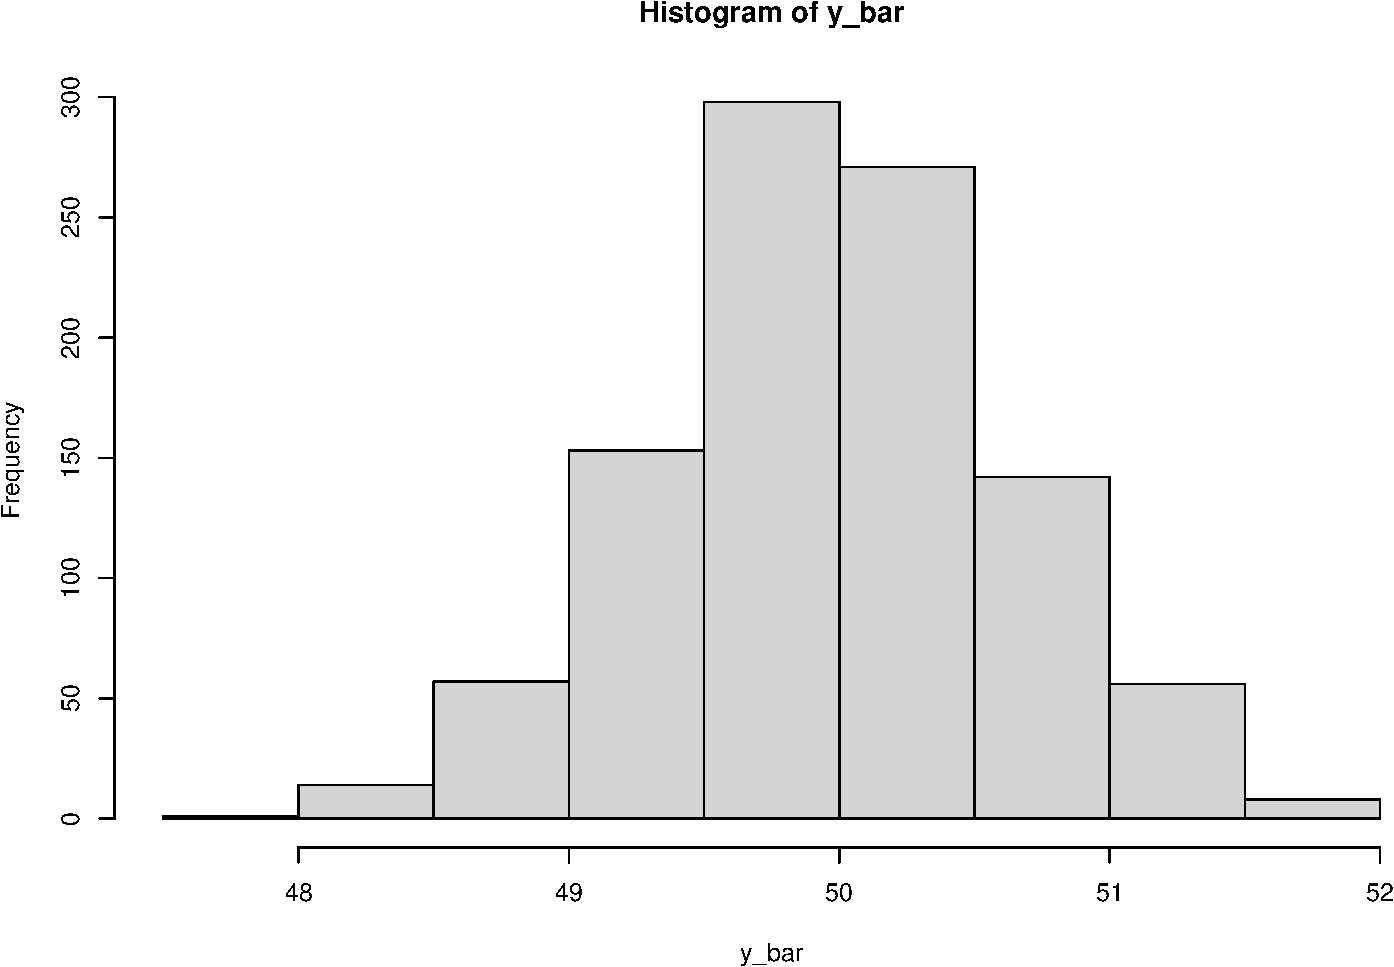
\includegraphics[keepaspectratio]{part2_inclass_files/figure-beamer/unnamed-chunk-11-1.pdf}}
\end{frame}

\begin{frame}[fragile]{Central Limit Theorem: Simulation}
\protect\phantomsection\label{central-limit-theorem-simulation-2}
Let's say that we take many samples of size 20 from the population. We
would expect \(\bar{Y}\) to be approximately normal with mean 50 and
variance 16/20 = 0.8.

\begin{itemize}
\tightlist
\item
  \texttt{replicate()}: repeat an expression n times (different n from
  \texttt{rnorm})
\item
  \texttt{apply()}: for each column (MARGIN = 2), apply the mean
  function
\end{itemize}

\begin{Shaded}
\begin{Highlighting}[]
\FunctionTok{mean}\NormalTok{(y\_bar)}
\end{Highlighting}
\end{Shaded}

\begin{verbatim}
[1] 49.97217
\end{verbatim}

\begin{Shaded}
\begin{Highlighting}[]
\FunctionTok{var}\NormalTok{(y\_bar)}
\end{Highlighting}
\end{Shaded}

\begin{verbatim}
[1] 0.4365369
\end{verbatim}

\begin{Shaded}
\begin{Highlighting}[]
\FunctionTok{sd}\NormalTok{(y\_bar)}
\end{Highlighting}
\end{Shaded}

\begin{verbatim}
[1] 0.6607094
\end{verbatim}
\end{frame}

\begin{frame}{Central Limit Theorem: Example}
\protect\phantomsection\label{central-limit-theorem-example}
Suppose that you are estimating the average weight of sheep in a large
herd. You obtain a random sample of size \(n=50\), and can assume that
\(\mu=40\) and \(\sigma^2=4\). What is the probability that the sample
mean will be within 0.1 pounds of \(\mu\)?

\[
\bar{Y}\approx 
\]
\end{frame}

\begin{frame}[fragile]{Central Limit Theorem: Example}
\protect\phantomsection\label{central-limit-theorem-example-1}
\[
P(39.9\leq \bar{Y} \leq 40.1)
\] \textbf{Standard Normal Distribution}

\begin{Shaded}
\begin{Highlighting}[]
\FunctionTok{pnorm}\NormalTok{((}\FloatTok{40.1}\DecValTok{{-}40}\NormalTok{) }\SpecialCharTok{/} \FunctionTok{sqrt}\NormalTok{(}\DecValTok{4}\SpecialCharTok{/}\DecValTok{50}\NormalTok{)) }\SpecialCharTok{{-}} \FunctionTok{pnorm}\NormalTok{((}\FloatTok{39.9}\DecValTok{{-}40}\NormalTok{) }\SpecialCharTok{/} \FunctionTok{sqrt}\NormalTok{(}\DecValTok{4}\SpecialCharTok{/}\DecValTok{50}\NormalTok{))}
\end{Highlighting}
\end{Shaded}

\begin{verbatim}
[1] 0.2763264
\end{verbatim}

\textbf{Normal Distribution}

\begin{Shaded}
\begin{Highlighting}[]
\FunctionTok{pnorm}\NormalTok{(}\FloatTok{40.1}\NormalTok{, }\AttributeTok{mean =} \DecValTok{40}\NormalTok{, }\AttributeTok{sd =} \FunctionTok{sqrt}\NormalTok{(}\DecValTok{4}\SpecialCharTok{/}\DecValTok{50}\NormalTok{)) }\SpecialCharTok{{-}} \FunctionTok{pnorm}\NormalTok{(}\FloatTok{39.9}\NormalTok{, }\AttributeTok{mean =} \DecValTok{40}\NormalTok{, }\AttributeTok{sd =} \FunctionTok{sqrt}\NormalTok{(}\DecValTok{4}\SpecialCharTok{/}\DecValTok{50}\NormalTok{)) }
\end{Highlighting}
\end{Shaded}

\begin{verbatim}
[1] 0.2763264
\end{verbatim}
\end{frame}

\begin{frame}{Poisson Distribution}
\protect\phantomsection\label{poisson-distribution}
Poisson distribution is used to model the number of occurrences of
``rare'' events in certain intervals of time and space. A Poisson random
variable is a discrete random variable as it represents a count.

\[
P(X=x)=\frac{e^{-\lambda}\lambda^x}{x!}; \quad x=0,1,2,3,\dots
\]

where \(\lambda\) is the mean parameter and represents the expected
number of events occurring in the interval of interest.
\end{frame}

\begin{frame}{Poisson Distribution Examples}
\protect\phantomsection\label{poisson-distribution-examples}
\begin{itemize}
\item
  \(X\) = \# of alpha particles emitted from a polonium bar in an 8
  minute period\\
\item
  \(Y\) = \# of flaws on a standard size piece of manufactured product
  (e.g., 100m coaxial cable, 100 sq.meter plastic sheeting)\\
\item
  \(Z\) = \# of hits on a web page in a 24h period
\end{itemize}
\end{frame}

\begin{frame}{Poisson Distribution Properties}
\protect\phantomsection\label{poisson-distribution-properties}
Let \(X\sim Poi(\lambda)\).

\begin{itemize}
\tightlist
\item
  E(X) =
\end{itemize}

\hfill\break
\hfill\break
\hfill\break

\begin{itemize}
\tightlist
\item
  V(X) =
\end{itemize}

\hfill\break
\hfill\break
\hfill\break

\begin{itemize}
\tightlist
\item
  If \(X_i\sim Poi(\lambda)\) for \(i=1,2,\dots,n\), then
  \(\sum_{i=1}^n X_i \sim Poi(n\lambda)\)
\end{itemize}
\end{frame}

\begin{frame}[fragile]{Poisson Distribution: R}
\protect\phantomsection\label{poisson-distribution-r}
Let \(X\sim Poi(\lambda)\).

\begin{itemize}
\tightlist
\item
  \(P(X = x)\): \texttt{dpois(x=x,\ lambda=lambda)}
\end{itemize}

\hfill\break
\hfill\break
\hfill\break

\begin{itemize}
\tightlist
\item
  \(P(X \leq x)\): \texttt{ppois(x=x,\ lambda=lambda)}
\end{itemize}
\end{frame}

\begin{frame}{Example problems}
\protect\phantomsection\label{example-problems}
Let \(\mu=10\) and \(n=30\). When required, approximate \(\sigma^2\)
using the variance formula of the Binomial distribution. Compute each of
the following problems for the Binomial, Normal, and Poisson
distributions, as well as for \(\bar{Y}\).

\begin{itemize}
\tightlist
\item
  \(P(X\leq 4)\)
\item
  \(P(X\lt 4)\)
\item
  \(P(12\leq X \leq 24)\)
\item
  \(x\) such that \(P(X\leq x)=0.025\)
\item
  \(x\) such that \(P(X>x)=0.0975\)
\end{itemize}
\end{frame}




\end{document}
